\usepackage{pgf}
\usepackage{tikz}
\usetikzlibrary{arrows,automata,plotmarks}
\usepackage{pgfplots}
\pgfplotsset{compat=1.15}

\tikzset{
    % node styles
    state-node/.style={
        fill=none, shape=circle, draw=black, thick, text=black, minimum size=0.6cm},
    action-node/.style={
        fill=black, draw=none, text=white, shape=circle, inner sep=0.05cm, minimum size=0.2cm},
    reward-node/.style={
        fill=none, draw=black, text=black},
    hidden-node/.style={
        fill=none, draw=none, text=white, shape=circle, inner sep=0,outer sep=0, minimum size=0.0cm},
    % label styles
    action-label/.style={
        shape=circle, text=white, draw=none, fill=black, inner sep=0.05cm, minimum size=0.2cm, align=center, yshift=0.0cm, anchor=center},
    reward-label/.style={
        shape=rectangle, text=black, draw=black, fill=white, minimum size=0.5cm, align=center, yshift=0.0cm, anchor=center},
    hidden-edge/.style={
        text=white, draw=none, fill=none, inner sep=0,outer sep=0, minimum size=0.0cm},
}


% Diagrama de interação
\newcommand{\rlinteraction}{
    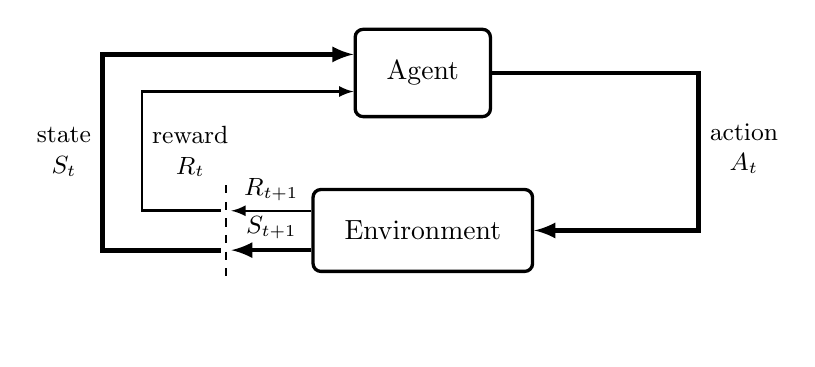
\begin{tikzpicture}[->,>=latex, auto, node distance=2.0cm, very thick, font=\small]
        \tikzstyle{rect-node}=[fill=none,shape=rectangle,draw=black,text=black,rounded corners=0.1cm, inner sep=0.4cm]
        \tikzstyle{hidden-node}=[fill=none, draw=none, text=black, shape=rectangle, inner sep=0,outer sep=0.05cm, minimum height=0.75cm]
        
        \node[rect-node]  (Agent)                                     {\normalsize Agent};
        \node[rect-node]  (Env)     [below of=Agent]                  {\normalsize Environment};
        \node[hidden-node] (Hidden)  [left of=Env, xshift=-0.5cm]     {};
        \node[hidden-node] (UpHid)   [above of=Hidden, yshift=-1.0cm] {};
        \node[hidden-node] (DownHid) [below of=Hidden, yshift=1.0cm]  {};
        
        \draw[thick, transform canvas={yshift=0.25cm}] (Env) to node[above] 
            {$R_{t+1}$} (Hidden);
        \draw[ultra thick, transform canvas={yshift=-0.25cm}] (Env) to node[above] 
            {$S_{t+1}$} (Hidden);
        \draw[ultra thick] (Hidden.255) to node[left, pos=1.0, yshift=1.25cm, align=center] 
            {state\\$S_t$}  ++(-1.5,0) |- (Agent.165);
        \draw[thick] (Hidden.105) to node[right, pos=1.0, yshift=0.75cm, align=center] 
            {reward\\$R_t$} ++(-1.0,0) |- (Agent.195);
        \draw[ultra thick] (Agent) to node[below right, pos=1.0, yshift=-0.5cm, align=center] 
            {action\\$A_t$} ++(3.5,0)  |- (Env);
        \draw[-, thick, dashed] (UpHid) to node {} (DownHid);
    \end{tikzpicture}
}


\newcommand{\rlinteractionpomdp}{
    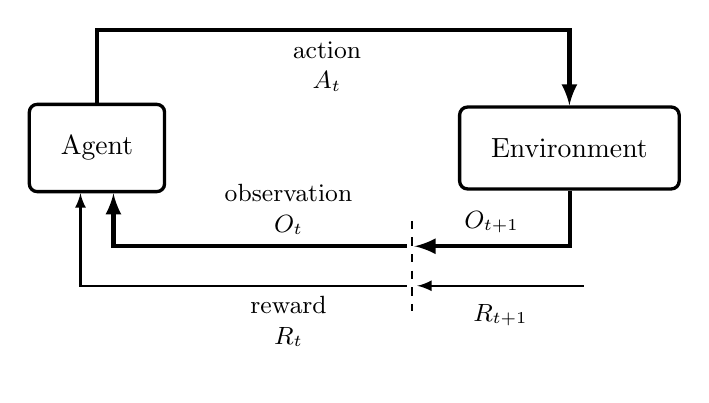
\begin{tikzpicture}[->,>=latex, auto, node distance=2.0cm, very thick, font=\small]
        \tikzstyle{rect-node}=[fill=none,shape=rectangle,draw=black,text=black,rounded corners=0.1cm, inner sep=0.4cm]
        \tikzstyle{hidden-node}=[fill=none, draw=none, text=black, shape=rectangle, inner sep=0,outer sep=0.05cm, minimum height=0.75cm]
        
        \node[rect-node] (Agent) {\normalsize Agent};
        \node[rect-node] (Env) [right of=Agent, xshift=4.0cm] {\normalsize Environment};
        \node[hidden-node] (Hidden) [below of=Env, xshift=-2.0cm, yshift=0.5cm] {};
        \node[hidden-node] (UpHid) [above of=Hidden, yshift=-1.0cm] {};
        \node[hidden-node] (DownHid) [below of=Hidden, yshift=1.0cm] {};
        \node[hidden-node] (Reward) [below of=Env, xshift=0.25cm, yshift=0.5cm] {};
        
        \draw[thick, transform canvas={yshift=-0.25cm}] (Reward) to node[below, yshift=-0.1cm] 
            {$R_{t+1}$} (Hidden);
            
        \draw[ultra thick, transform canvas={xshift=0.10cm}] (Env.260) to node[xshift=-0.5cm, yshift=-0.4cm] {$O_{t+1}$} ++(0,0) |- (Hidden.105);
            
        \draw[ultra thick] (Hidden.105) to node[above, xshift=-1.5cm, align=center] 
            {observation\\$O_t$}  ++(0,0) -| (Agent.290);
        \draw[thick] (Hidden.255) to node[below, xshift=-1.5cm, align=center] 
            {reward\\$R_t$} ++(0,0) -| (Agent.250);
            
        \draw[ultra thick] (Agent) to node[xshift=3.5cm, align=center] 
            {action\\$A_t$} ++(0,1.5) -| (Env);
            
        \draw[-, thick, dashed] (UpHid) to node {} (DownHid);
    \end{tikzpicture}
}


\newcommand{\mdpthreestate}{
    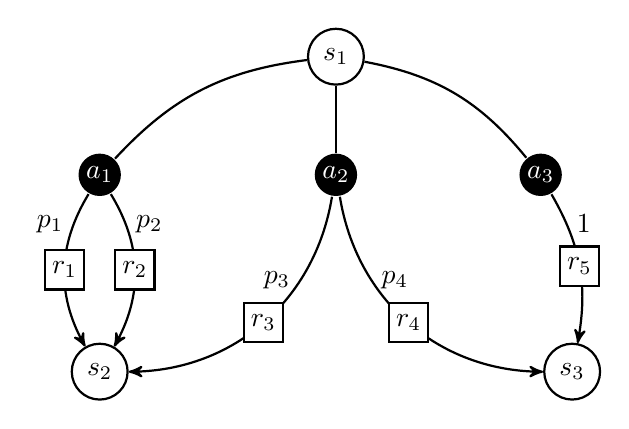
\begin{tikzpicture}[->,>=stealth', auto, node distance=4.0cm, thick]
        \node[state-node]  (S1) {$s_1$};
        \node[state-node]  (S2) [below of=S1, xshift=-3.0cm] {$s_2$};
        \node[state-node]  (S3) [below of=S1, xshift= 3.0cm] {$s_3$};
        \node[action-node] (A1) [below of=S1, yshift=2.5cm, xshift=-3.0cm] {$a_1$};
        \node[action-node] (A2) [below of=S1, yshift=2.5cm]  {$a_2$};
        \node[action-node] (A3) [below of=S1, yshift=2.5cm, xshift=2.6cm] {$a_3$};
        
        \draw[bend right=20,-] (S1) to node[]  {} (A1);
        \draw[-]               (S1) to node[]  {} (A2);
        \draw[bend left=20,-] (S1) to node[]  {} (A3);
        
        \draw[bend right=30]   (A1) to node[left, pos=0.2]  {$p_1$} (S2);
        \draw[bend left=30]    (A1) to node[right, pos=0.2] {$p_2$} (S2);
        \draw[bend left=40]    (A2) to node[left, pos=0.3]  {$p_3$} (S2);
        \draw[bend right=40]   (A2) to node[right, pos=0.3] {$p_4$} (S3);
        \draw[bend left=20]    (A3) to node[right, pos=0.2] {$1$} (S3);
        
        \draw[hidden-edge, bend right=30] (A1) to node[reward-label] {$r_1$} (S2);
        \draw[hidden-edge, bend left=30]  (A1) to node[reward-label] {$r_2$} (S2);
        \draw[hidden-edge, bend left=40]  (A2) to node[reward-label] {$r_3$} (S2);
        \draw[hidden-edge, bend right=40] (A2) to node[reward-label] {$r_4$} (S3);
        \draw[hidden-edge, bend left=20]  (A3) to node[reward-label] {$r_5$} (S3);
    \end{tikzpicture}
}

\newcommand{\mdpthreestatenoprobs}{
    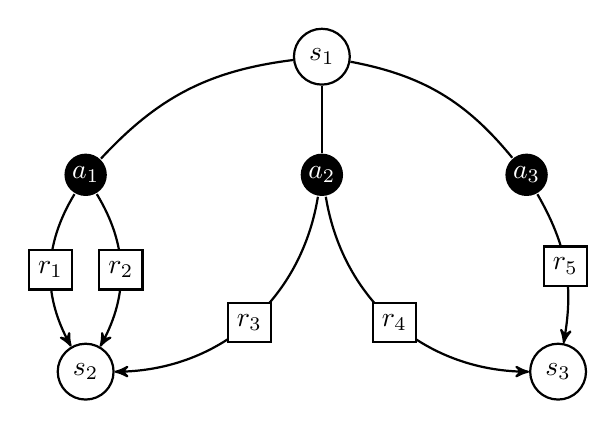
\begin{tikzpicture}[->,>=stealth', auto, node distance=4.0cm, thick]
        \node[state-node]  (S1) {$s_1$};
        \node[state-node]  (S2) [below of=S1, xshift=-3.0cm] {$s_2$};
        \node[state-node]  (S3) [below of=S1, xshift= 3.0cm] {$s_3$};
        \node[action-node] (A1) [below of=S1, yshift=2.5cm, xshift=-3.0cm] {$a_1$};
        \node[action-node] (A2) [below of=S1, yshift=2.5cm]  {$a_2$};
        \node[action-node] (A3) [below of=S1, yshift=2.5cm, xshift=2.6cm] {$a_3$};
        
        \draw[bend right=20,-] (S1) to node[]  {} (A1);
        \draw[-]               (S1) to node[]  {} (A2);
        \draw[bend left=20,-] (S1) to node[]  {} (A3);
        
        \draw[bend right=30] (A1) to node[reward-label] {$r_1$} (S2);
        \draw[bend left=30]  (A1) to node[reward-label] {$r_2$} (S2);
        \draw[bend left=40]  (A2) to node[reward-label] {$r_3$} (S2);
        \draw[bend right=40] (A2) to node[reward-label] {$r_4$} (S3);
        \draw[bend left=20]  (A3) to node[reward-label] {$r_5$} (S3);
    \end{tikzpicture}
}

\newcommand{\mdpbig}{
    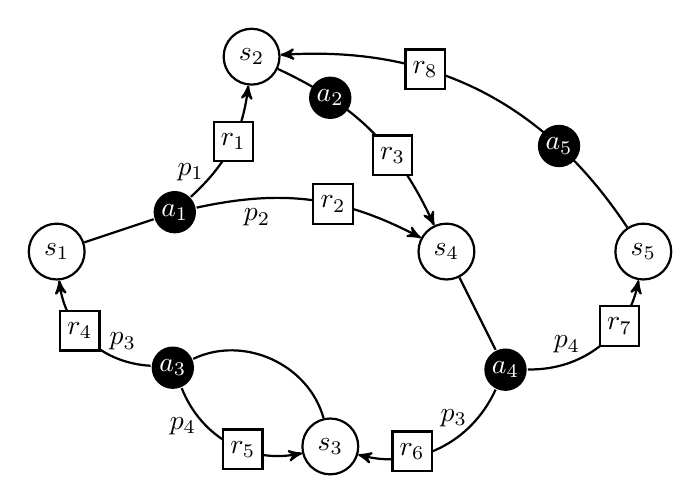
\begin{tikzpicture}[->,>=stealth',auto,node distance=3.5cm, thick]
        \node[state-node] (S1)                     {$s_1$};
        \node[state-node] (S2) [above right of=S1] {$s_2$};
        \node[state-node] (S3) [below right of=S1, xshift=1.0cm] {$s_3$};
        \node[state-node] (S4) [below right of=S2] {$s_4$};
        \node[state-node] (S5) [right of=S4, xshift=-1.0cm]       {$s_5$};
        
        \node[action-node] (A1) [right of=S1, xshift=-2.0cm, yshift=0.5cm] {$a_1$};
        \node[action-node] (A3) [left of=S3, xshift=1.5cm, yshift=1.0cm] {$a_3$};
        \node[action-node] (A4) [below of=S4, xshift=0.75cm, yshift=2.0cm] {$a_4$};
        
        % from (S1)
        \draw[-] (S1) to node[] {} (A1);
        \draw[bend right=20] (A1) to node[left, pos=0.25] {$p_1$} (S2);
        \draw[bend left=20] (A1) to node[below, pos=0.25] {$p_2$} (S4);
        \draw[hidden-edge, bend right=20] (A1) to node[reward-label, pos=0.55] {$r_1$} (S2);
        \draw[hidden-edge, bend left=20] (A1) to node[reward-label, pos=0.60] {$r_2$} (S4);
        
        % from (S2)
        \draw[bend left=20] (S2) to node[action-label, pos=0.25] {$a_2$} (S4);
        \draw[hidden-edge, bend left=20] (S2) to node[reward-label, pos=0.65] {$r_3$} (S4);
        
        % from (S3)
        \draw[-, bend right=50] (S3) to node[] {} (A3);
        \draw[bend left=40] (A3) to node[above, pos=0.2] {$p_3$} (S1);
        \draw[bend right=40] (A3) to node[left, pos=0.3] {$p_4$} (S3);
        \draw[hidden-edge, bend left=40] (A3) to node[reward-label, pos=0.6] {$r_4$} (S1);
        \draw[hidden-edge, bend right=40] (A3) to node[reward-label, pos=0.6] {$r_5$} (S3);
        
        % from (S4)
        \draw[-] (S4) to node[] {} (A4);
        \draw[bend left=40] (A4) to node[left, pos=0.2] {$p_3$} (S3);
        \draw[bend right=40] (A4) to node[above, pos=0.25] {$p_4$} (S5);
        \draw[hidden-edge, bend left=40] (A4) to node[reward-label, left, pos=0.55] {$r_6$} (S3);
        \draw[hidden-edge, bend right=40] (A4) to node[reward-label, above right, pos=0.5] {$r_7$} (S5);
        
        % from (S5)
        \draw[bend right] (S5) to node[action-label, pos=0.25] {$a_5$} (S2);
        \draw[hidden-edge, bend right] (S5) to node[reward-label, pos=0.65] {$r_8$} (S2);
        
    \end{tikzpicture}
}


\newcommand{\simplebandit}{
    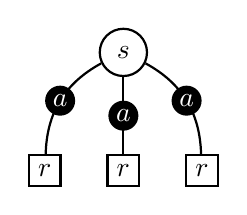
\begin{tikzpicture}[-,>=stealth', auto, node distance=1.5cm, thick]
        \node[state-node]  (SimpleBanditS1) {$s$};
        \node[reward-node] (SimpleBanditR1) [below of=SimpleBanditS1, xshift=-1.0cm] {$r$};
        \node[reward-node] (SimpleBanditR2) [below of=SimpleBanditS1, xshift=0.0cm]  {$r$};
        \node[reward-node] (SimpleBanditR3) [below of=SimpleBanditS1, xshift=1.0cm]  {$r$};
        
        \draw[bend right] (SimpleBanditS1) to node[action-label] {$a$} (SimpleBanditR1);
        \draw             (SimpleBanditS1) to node[action-label] {$a$} (SimpleBanditR2);
        \draw[bend left]  (SimpleBanditS1) to node[action-label] {$a$} (SimpleBanditR3);
    \end{tikzpicture}
}

\newcommand{\associativebandits}{
    \begin{tikzpicture}[thick]
        \node[draw=black] (AB1) {
            \begin{tikzpicture}[]
                \node[] (B1) {
                    \simplebandit
                };
                \node[right of=B1, xshift=2.0cm] (B2) {
                    \simplebandit
                };
                \node[right of=B2, xshift=2.0cm] (B3) {
                    \simplebandit
                };
                \node[right of=B3, xshift=1.0cm] (B4) {
                    $\boldsymbol{\cdots}$
                };
                \node[right of=B4, xshift=1.0cm] (B5) {
                    \simplebandit
                };
            \end{tikzpicture}
        };
        
        \node[draw=black, below of=AB1, yshift=-2.0cm] (AB2) {
            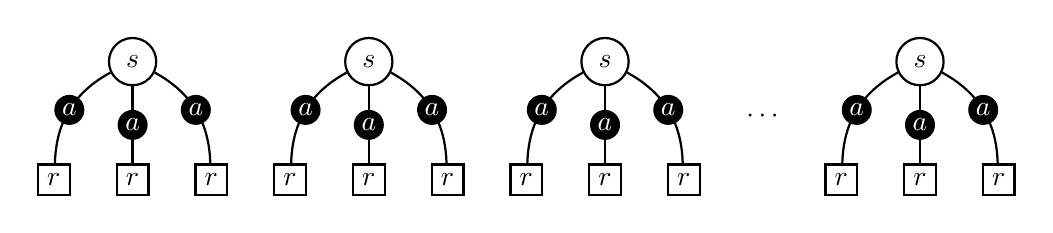
\begin{tikzpicture}[]
                \node[] (B1) {
                    \simplebandit
                };
                \node[right of=B1, xshift=2.0cm] (B2) {
                    \simplebandit
                };
                \node[right of=B2, xshift=2.0cm] (B3) {
                    \simplebandit
                };
                \node[right of=B3, xshift=1.0cm] (B4) {
                    $\boldsymbol{\cdots}$
                };
                \node[right of=B4, xshift=1.0cm] (B5) {
                    \simplebandit
                };
            \end{tikzpicture}
        };
        
        \node[below of=AB2, yshift=-1.0cm] (AB3) {
            $\Huge\vdots$
        };
    
        \node[draw=black, below of=AB3, yshift=-1.0cm] (AB4) {
            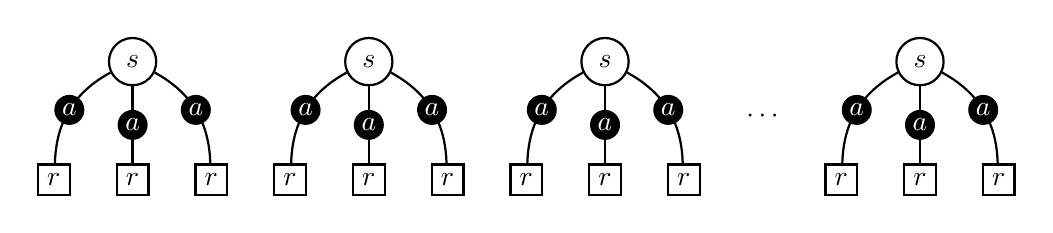
\begin{tikzpicture}[]
                \node[] (B1) {
                    \simplebandit
                };
                \node[right of=B1, xshift=2.0cm] (B2) {
                    \simplebandit
                };
                \node[right of=B2, xshift=2.0cm] (B3) {
                    \simplebandit
                };
                \node[right of=B3, xshift=1.0cm] (B4) {
                    $\boldsymbol{\cdots}$
                };
                \node[right of=B4, xshift=1.0cm] (B5) {
                    \simplebandit
                };
            \end{tikzpicture}
        };
        
        \draw[->, thick] (AB1) to node {} (AB2);
        \draw[->, thick] (AB2) to node {} (AB3);
        \draw[->, thick] (AB3) to node {} (AB4);
    \end{tikzpicture}
}

\newcommand{\fullrldiagram}{
    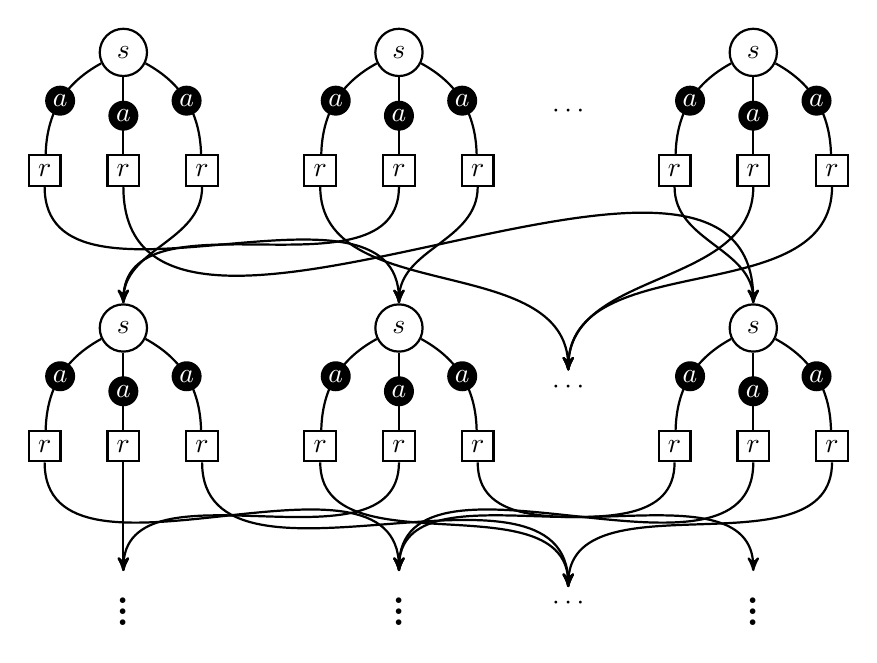
\begin{tikzpicture}[-,>=stealth', auto, node distance=1.5cm, thick]
        \node[state-node] (S1) {$s$};
        \node[reward-node] (R1S1) [below of=S1, xshift=-1.0cm] {$r$};
        \node[reward-node] (R2S1) [below of=S1]                {$r$};
        \node[reward-node] (R3S1) [below of=S1, xshift=1.0cm]  {$r$};
        
        \draw[bend right] (S1) to node[action-label] {$a$} (R1S1);
        \draw[]           (S1) to node[action-label] {$a$} (R2S1);
        \draw[bend left]  (S1) to node[action-label] {$a$} (R3S1);
        
        \node[state-node] (S2) [right of=S1, xshift=2.0cm] {$s$};
        \node[reward-node] (R1S2) [below of=S2, xshift=-1.0cm] {$r$};
        \node[reward-node] (R2S2) [below of=S2]                {$r$};
        \node[reward-node] (R3S2) [below of=S2, xshift=1.0cm]  {$r$};
        
        \draw[bend right] (S2) to node[action-label] {$a$} (R1S2);
        \draw[]           (S2) to node[action-label] {$a$} (R2S2);
        \draw[bend left]  (S2) to node[action-label] {$a$} (R3S2);
        
        \node[right of=S2, xshift=0.65cm, yshift=-0.75cm] (DOTS1) {
            $\boldsymbol{\cdots}$
        };
        
        \node[state-node] (S3) [right of=S2, xshift=3.0cm] {$s$};
        \node[reward-node] (R1S3) [below of=S3, xshift=-1.0cm] {$r$};
        \node[reward-node] (R2S3) [below of=S3]                {$r$};
        \node[reward-node] (R3S3) [below of=S3, xshift=1.0cm]  {$r$};
        
        \draw[bend right] (S3) to node[action-label] {$a$} (R1S3);
        \draw[]           (S3) to node[action-label] {$a$} (R2S3);
        \draw[bend left]  (S3) to node[action-label] {$a$} (R3S3);
        
        
        \node[state-node] (S4) [below of=S1, yshift=-2.0cm] {$s$};
        \node[reward-node] (R1S4) [below of=S4, xshift=-1.0cm] {$r$};
        \node[reward-node] (R2S4) [below of=S4]                {$r$};
        \node[reward-node] (R3S4) [below of=S4, xshift=1.0cm]  {$r$};
        
        \draw[bend right] (S4) to node[action-label] {$a$} (R1S4);
        \draw[]           (S4) to node[action-label] {$a$} (R2S4);
        \draw[bend left]  (S4) to node[action-label] {$a$} (R3S4);
        
        \node[state-node] (S5) [right of=S4, xshift=2.0cm] {$s$};
        \node[reward-node] (R1S5) [below of=S5, xshift=-1.0cm] {$r$};
        \node[reward-node] (R2S5) [below of=S5]                {$r$};
        \node[reward-node] (R3S5) [below of=S5, xshift=1.0cm]  {$r$};
        
        \draw[bend right] (S5) to node[action-label] {$a$} (R1S5);
        \draw[]           (S5) to node[action-label] {$a$} (R2S5);
        \draw[bend left]  (S5) to node[action-label] {$a$} (R3S5);
        
        \node[right of=S5, xshift=0.65cm, yshift=-0.75cm] (DOTS2) {$\boldsymbol{\cdots}$};
        
        \node[state-node] (S6) [right of=S5, xshift=3.0cm] {$s$};
        \node[reward-node] (R1S6) [below of=S6, xshift=-1.0cm] {$r$};
        \node[reward-node] (R2S6) [below of=S6]                {$r$};
        \node[reward-node] (R3S6) [below of=S6, xshift=1.0cm]  {$r$};
        
        \draw[bend right] (S6) to node[action-label] {$a$} (R1S6);
        \draw[]           (S6) to node[action-label] {$a$} (R2S6);
        \draw[bend left]  (S6) to node[action-label] {$a$} (R3S6);
        
        
        \draw[->, out=-90, in=90] (R1S1) to node[] {} (S5);
        \draw[->, out=-90, in=90] (R2S1) to node[] {} (S6);
        \draw[->, out=-90, in=90] (R3S1) to node[] {} (S4);
        
        \draw[->, out=-90, in=90] (R1S2) to node[] {} (DOTS2);
        \draw[->, out=-90, in=90] (R2S2) to node[] {} (S4);
        \draw[->, out=-90, in=90] (R3S2) to node[] {} (S5);
        
        \draw[->, out=-90, in=90] (R1S3) to node[] {} (S6);
        \draw[->, out=-90, in=90] (R2S3) to node[] {} (DOTS2);
        \draw[->, out=-90, in=90] (R3S3) to node[] {} (DOTS2);
        
        
        \node[below of=S4, yshift=-2.0cm] (DOTS3) {$\Huge\vdots$};
        \node[right of=DOTS3, xshift=2.0cm] (DOTS4) {$\Huge\vdots$};
        \node[right of=DOTS4, xshift=0.65cm] (DOTS5) {$\boldsymbol{\cdots}$};
        \node[right of=DOTS4, xshift=3.0cm] (DOTS6) {$\Huge\vdots$};
        
        
        \draw[->, out=-90, in=90] (R1S4) to node[] {} (DOTS4);
        \draw[->, out=-90, in=90] (R2S4) to node[] {} (DOTS3);
        \draw[->, out=-90, in=90] (R3S4) to node[] {} (DOTS5);
        
        \draw[->, out=-90, in=90] (R1S5) to node[] {} (DOTS5);
        \draw[->, out=-90, in=90] (R2S5) to node[] {} (DOTS3);
        \draw[->, out=-90, in=90] (R3S5) to node[] {} (DOTS6);
        
        \draw[->, out=-90, in=90] (R1S6) to node[] {} (DOTS4);
        \draw[->, out=-90, in=90] (R2S6) to node[] {} (DOTS4);
        \draw[->, out=-90, in=90] (R3S6) to node[] {} (DOTS5);
    \end{tikzpicture}
}